\section{Fusie en Splijting van Vortexknopen binnen VAM}

Wanneer we naar zwaardere knopen gaan, komt er een competitie tussen één knoop houden of opsplitsen in meerdere knopen. Dit is analoog aan kernen: lichte kernen fuseren exotherm (één grotere knoop is energetisch gunstiger), middelzware zijn het stabielst in hun eentje, en zeer zware kernen fissioneren (twee middelgrote knopen energetisch gunstiger dan één reuzenknoop).

% --- Figuur 3: Fusie vs Splitsing energie ---
\begin{figure}[H]
    \centering
    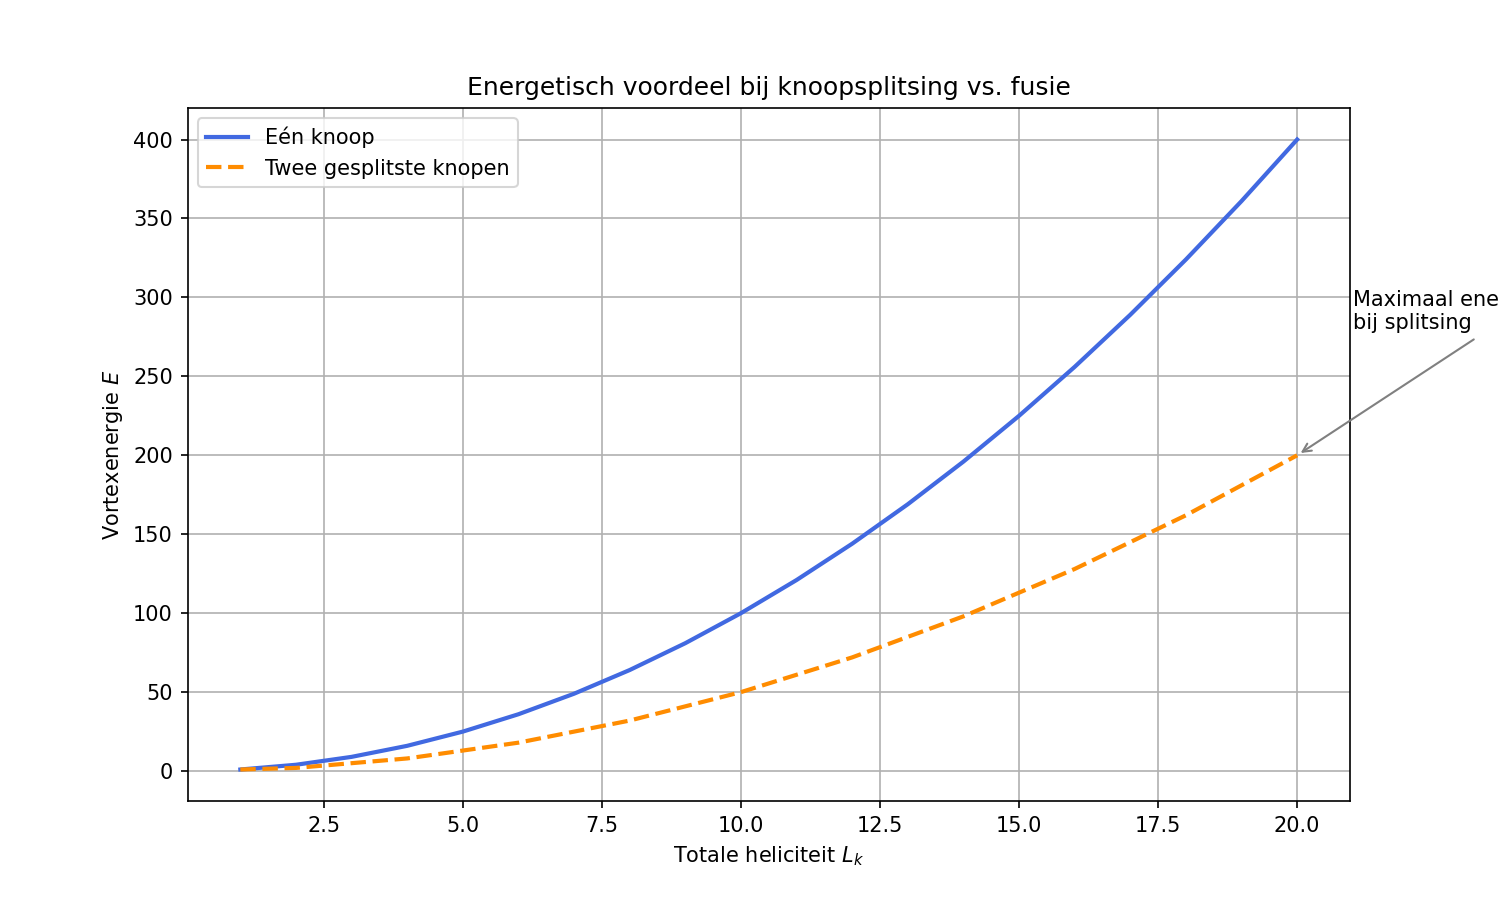
\includegraphics[width=0.7\textwidth]{sections/3_EnergetischVoordeel}
    \caption{Energievergelijking tussen een enkele vortexknoop en twee opgesplitste knopen met dezelfde totale heliciteit $L_k$. Splitsing verlaagt de totale vortexenergie.}
    \label{fig:fusie_splitsing}
\end{figure}

VAM levert een topologische interpretatie:

\textbf{Fusie:} Twee losse vortexknopen (bijv. twee $T(2,3)$ knopen voor 2 H) kunnen bij dicht bijeen brengen een overlappende wervelstructuur gaan delen en samensmelten tot één knoop van hogere $L_k$ (He met $T(2,5)$). Dit wordt vergemakkelijkt als de vorticiteit-geïnduceerde druk tussen de knopen de Coulomb-afstoting compenseert. VAM berekent dat bij kernafstand $\sim 2r_c$ een significante drukval $\Delta P$ optreedt die de effectieve barrière verlaagt – een hydrodynamische kijk op quantum tunneling. Knoopfusie is dus energetisch voordelig zolang de resulterende knoop voldoende onderdruk creëert om stabiel te zijn. Dit stopt rond ijzer: daarna voegt extra $L_k$ zoveel rotatie-energie toe dat de onderdruk per nucleon minder wordt (de knoop wordt “te strak opgekruld” en verliest relatieve stabiliteit).

\textbf{Splijting (fissie):} Een zeer complexe knoop (hoog $L_k$, groot $p$) kan energetisch winnen door in twee of meer knopen met lagere $L_k$
te splitsen. Topologisch vereist dit dat ergens het vortexveld breekt en herverbindt (reconnection)~\cite{Kleckner2013KnotsVortex} – normaal verboden in een ideale vloeistof, maar in werkelijkheid mogelijk via quantumfluïdum-effecten of extreme excitatie.
% --- Figuur 7: Reconnectie sequentie ---
\begin{figure}[H]
    \centering
    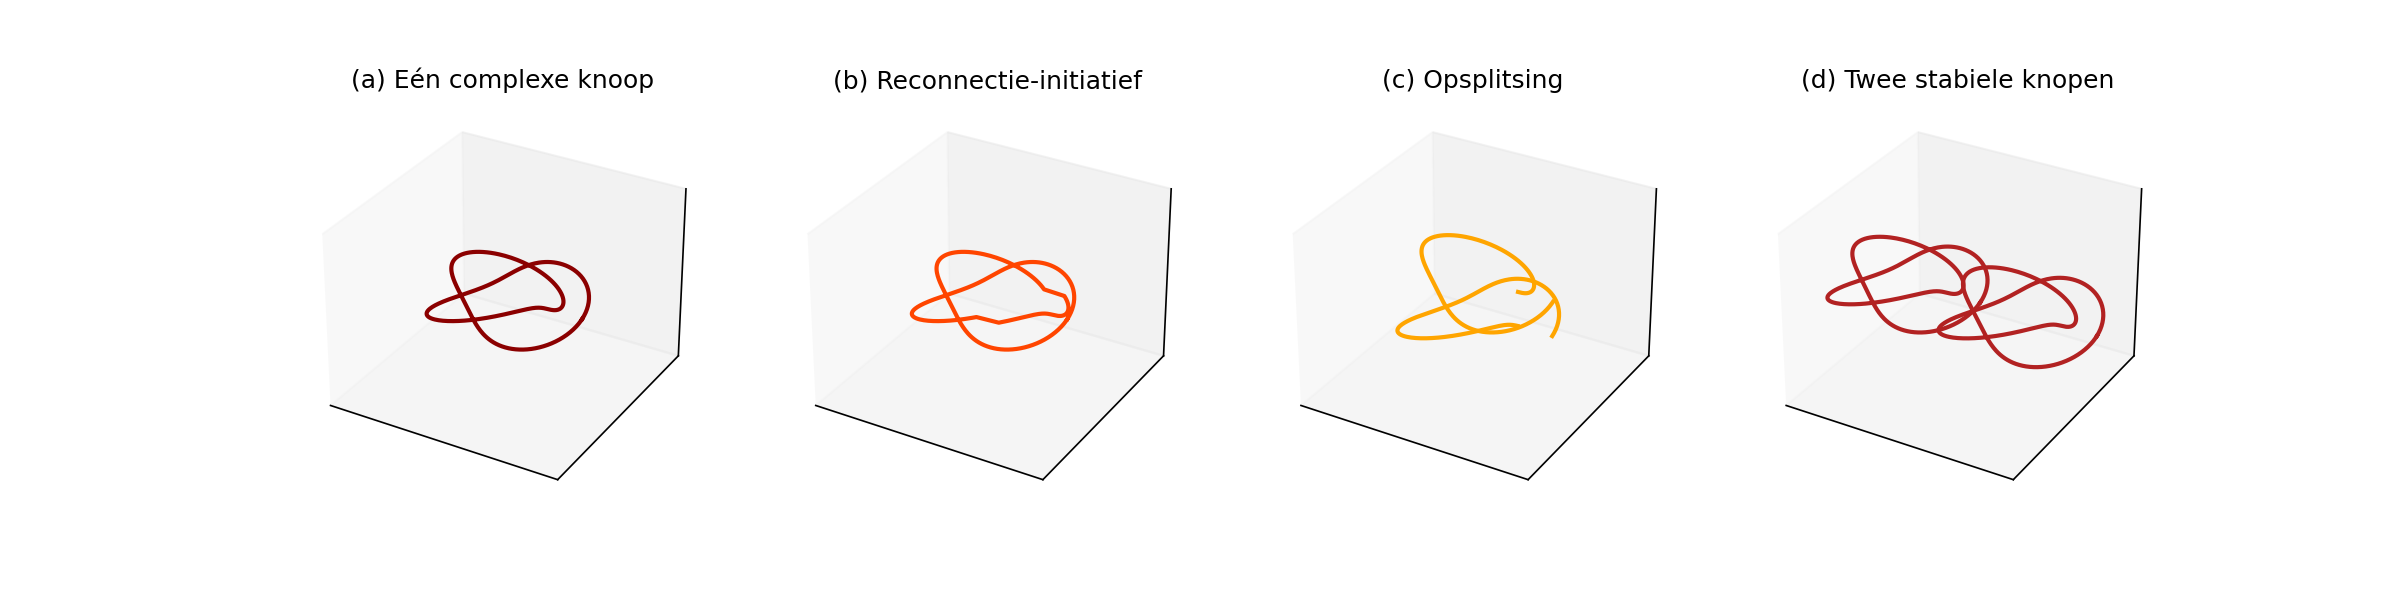
\includegraphics[width=0.85\textwidth]{sections/7_Slijten_Verbinden}
    \caption{Sequentiële weergave van vortexsplijting: een enkele knoop raakt topologisch instabiel en reconvergeert tot twee aparte knopen.}
    \label{fig:reconnectie_splijting}
\end{figure}

Uranium bijvoorbeeld kan via een zeldzame fluctuatieresonantie twee deelknooppatronen vormen (bijv. $T(3,q_1)$ en $T(3,q_2)$) die samen een lagere totale $H$ hebben dan de oorspronkelijke ($H$ blijft behouden maar verdeelt zich over fragmenten, vergelijkbaar met behoud van baryongetal bij splitsing). Omdat elke fragmentknoop een sterkere eigen binding heeft (minder spanning dan één superknoop), is dit energetisch gunstig en gebeurt het spontaan (radioactief verval). Binnen VAM zou men dit beschrijven als een knoop-naar-multiknoop resonantie: de zware knoop oscilleert naar een toestand waar een topologische “brug” vormt en splitst, analoog aan zeepbel-deelvorming of vortex ring splittings, zij het op quantum-schaal.

Kortom, de stabiliteit van elk element binnen VAM kan kwalitatief verklaard worden: lichte en middellange elementen blijven één torusknoop dankzij topologische inertie en vorticiteitsdruk; hele zware elementen naderen de grens waarbij multi-knoop configuraties winnen. Deze omslag is continu en onder voorwaarden – bijvoorbeeld neutronrijke isotopen (veel satellietknopen) verkleinen de onderlinge koppeling van de hoofdknoop, wat eerder tot instabiliteit leidt. We zien dit doordat isotopen met te veel of te weinig neutronen sneller vervallen. VAM zou dit kwantitatief kunnen modelleren via de entropie van vortexknopen (in eerdere VAM-werk is aangetoond dat men met Clausius-entropie aan vortexknopen thermodynamische consistentie krijgt). Een stabiele knoop is dus ook een entropisch minimum voor het gegeven $H$: er is geen configuratie met dezelfde heliciteit die lagere energie heeft. Wanneer die er wel is (bij zware kernen: twee knopen met ieder lagere heliciteit), dan treedt verval op.